\documentclass[tikz]{standalone}

%\usepackage[charter]{mathdesign}
\usepackage{newtxtext}
\usepackage{newtxmath}

\begin{document}

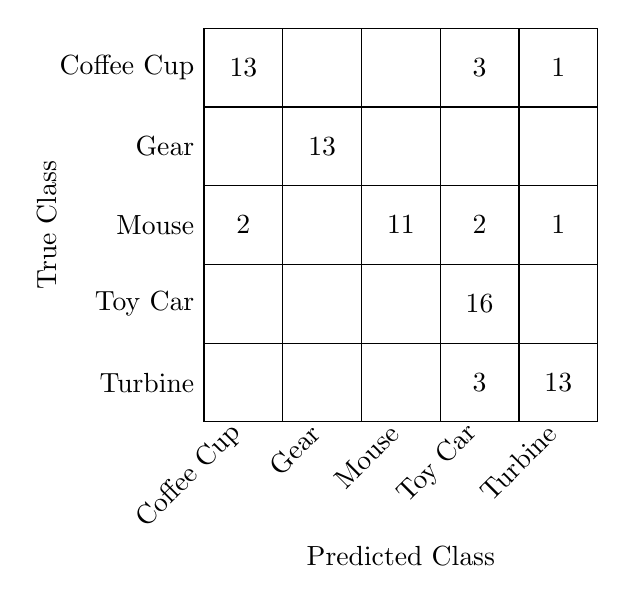
\begin{tikzpicture}

  \foreach \i in {0,...,5} {
    \draw[] (\i,0) -- (\i,5);
    \draw[] (0,\i) -- (5,\i);
  }

  \node[anchor=east] at (0,0.5) {Turbine};
  \node[anchor=east] at (0,1.5) {Toy Car};
  \node[anchor=east] at (0,2.5) {Mouse};
  \node[anchor=east] at (0,3.5) {Gear};
  \node[anchor=east] at (0,4.5) {Coffee Cup};

  \node[anchor=east, rotate=45] at (0.5,0) {Coffee Cup};
  \node[anchor=east, rotate=45] at (1.5,0) {Gear};
  \node[anchor=east, rotate=45] at (2.5,0) {Mouse};
  \node[anchor=east, rotate=45] at (3.5,0) {Toy Car};
  \node[anchor=east, rotate=45] at (4.5,0) {Turbine};

  \node[rotate=90] at (-2,2.5) {True Class};
  \node[] at (2.5,-1.7) {Predicted Class};

  \node[] at (0.5,4.5) {13};
  \node[] at (1.5,3.5) {13};
  \node[] at (2.5,2.5) {11};
  \node[] at (3.5,1.5) {16};
  \node[] at (4.5,0.5) {13};

  \node[] at (0.5,2.5) {2};
  \node[] at (3.5,0.5) {3};
  \node[] at (3.5,2.5) {2};
  \node[] at (3.5,4.5) {3};
  \node[] at (4.5,2.5) {1};
  \node[] at (4.5,4.5) {1};

\end{tikzpicture}

\end{document}
